\documentclass[french]{article}
\usepackage[T1]{fontenc}
\usepackage[utf8]{inputenc}
\usepackage[french]{babel}
\usepackage{amsmath}
\usepackage{mathtools}
\usepackage{color}
\usepackage[svgnames,dvipsnames]{xcolor} 
\usepackage{soul}
\usepackage{amssymb}
\usepackage{enumitem}
\usepackage{multicol}
\usepackage[left=2cm,right=2cm,top=2cm,bottom=2cm]{geometry}
\newcommand{\mathcolorbox}[2]{\colorbox{#1}{$\displaystyle #2$}}
\usepackage{pifont}
\usepackage{pst-all}
\usepackage{pstricks}
\usepackage{delarray}
\usepackage{setspace}
\usepackage{graphicx}
\usepackage{hyperref}
\usepackage{nicematrix}
\usepackage{listings}
\usepackage{float}

\hypersetup{
	colorlinks=true,
	linkcolor=blue,
	filecolor=magenta,      
	urlcolor=cyan,
	pdfpagemode=FullScreen,
}

\usepackage{amsthm}
\newtheorem*{Rem}{Remarque}

\newenvironment{conclusion}[1]{%
	\begin{center}\normalfont\textbf{Conclusion}\end{center}
	\begin{quotation} #1 \end{quotation}
}{%
	\vspace{1cm}
}

\newcommand\pythonstyle{\lstset{
	language=Python,
	basicstyle=\ttm,
	morekeywords={self},              % Add keywords here
	keywordstyle=\ttb\color{deepblue},
	emph={MyClass,__init__},          % Custom highlighting
	emphstyle=\ttb\color{deepred},    % Custom highlighting style
	stringstyle=\color{deepgreen},
	frame=tb,                         % Any extra options here
	showstringspaces=false
}}

\lstdefinestyle{Cpp}{
	language=C++,
	tabsize=3,
	basicstyle=\ttfamily,
	keywordstyle=\color{blue}\ttfamily,
	stringstyle=\color{red}\ttfamily,
	commentstyle=\color{green}\ttfamily,
	morecomment=[l][\color{magenta}]{\#}
}

\lstdefinestyle{Python}{
	language=Python,
	tabsize=3,
	basicstyle=\ttfamily,
	keywordstyle=\color{blue}\ttfamily,
	stringstyle=\color{red}\ttfamily,
	commentstyle=\color{green}\ttfamily,
	morecomment=[l][\color{magenta}]{\#}
}

\lstset{style=Cpp}

\setlength\parindent{0pt}
\usepackage[skip=2pt]{caption}

\usepackage{fontawesome}

\usepackage{lipsum}

\graphicspath{{images/}}

\usepackage[backend=biber,style=numeric,sorting=nyt]{biblatex}
\addbibresource{biblio.bib}



\begin{document}
	LECOURTIER Frédérique \hfill \today
	\begin{center}
		\Large\textbf{{Résultats}}
	\end{center}
	\tableofcontents
	\newpage

%	\nocite{*}

	\section{Étape 1 : Apprentissage d'une fonction Levelset $\phi$}
	
	\subsection{Génération des Inputs}
	
	On considère une courbe paramétrique $c(t)$ définissant un surface $\mathcal{S}$ (en 2D). En pratique, nous allons considérer les 3 formes définies par les courbes paramétriques, pour $t\in [0,1]$ :
	
	\begin{equation*}
		c_{circle}(t) = \begin{pmatrix}
			x_0 + r\cos(2\pi t) \\
			y_0 + r\sin(2\pi t)
		\end{pmatrix}, (x_0,y_0)=(0.5,0.5), r=\sqrt{2}/4
	\end{equation*}
	
	\begin{equation*}
		c_{bean}(t) = \begin{pmatrix}
			\sin(2\pi t) \times (\sin(2\pi t)^a+\cos(2\pi t)^b) \\
			-\cos(2\pi t) \times (\sin(2\pi t)^a+\cos(2\pi t)^b)
		\end{pmatrix}, a=3, b=5
	\end{equation*}

	\begin{equation*}
		c_{pumpkin}(t) = \begin{pmatrix}
			 \cos(2\pi t)+0.3\cos(6\pi t)+0.1\cos(10\pi t) \\
			 \sin(2\pi t)+0.3\sin(6\pi t)+0.1\sin(10\pi t)
		\end{pmatrix}
	\end{equation*}

	A partir de ces différentes courbes, on va générer un nombre $n_{bc}$ de points sur le surface $\mathcal{S}$ et on peut facilement calculer les normales à la surface en les points considérés. En considérants la dérivée $c'(t)$ de la courbe $c$ et $c'^{\perp}(t)$ définie comme la rotation de $c'$ d'un angle de $-\pi/2$, c'est-à-dire pour $\theta=\pi/2$, on a:
	\begin{equation*}
		c'^{\perp}(t) = \begin{pmatrix}
			\cos(\theta) & -\sin(\theta) \\
			\sin(\theta) & \cos(\theta)
		\end{pmatrix}c'(t)
	\end{equation*}
	et ainsi
	\begin{equation*}
		n(t)=\frac{c'^{\perp}(t)}{||c'^{\perp}(t)||}
	\end{equation*}
	
	\begin{minipage}{0.33\linewidth}
		\begin{figure}[H]
			\centering
			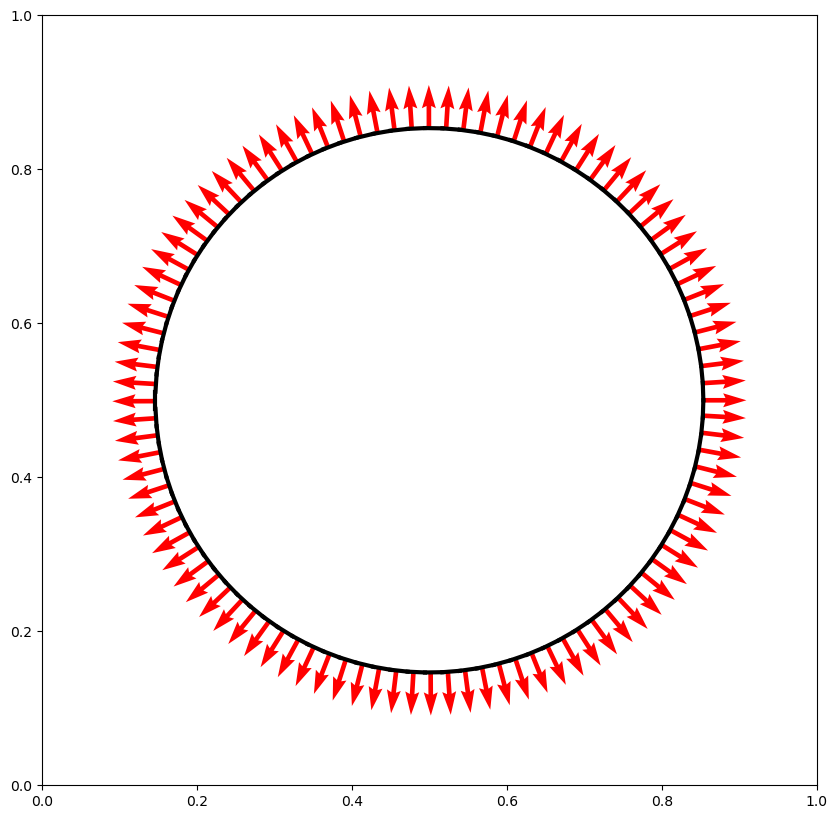
\includegraphics[width=\linewidth]{"levelset/circle/curve_circle.png"}
			\caption{Cercle.}
		\end{figure}
	\end{minipage}
	\begin{minipage}{0.33\linewidth}
		\begin{figure}[H]
			\centering
			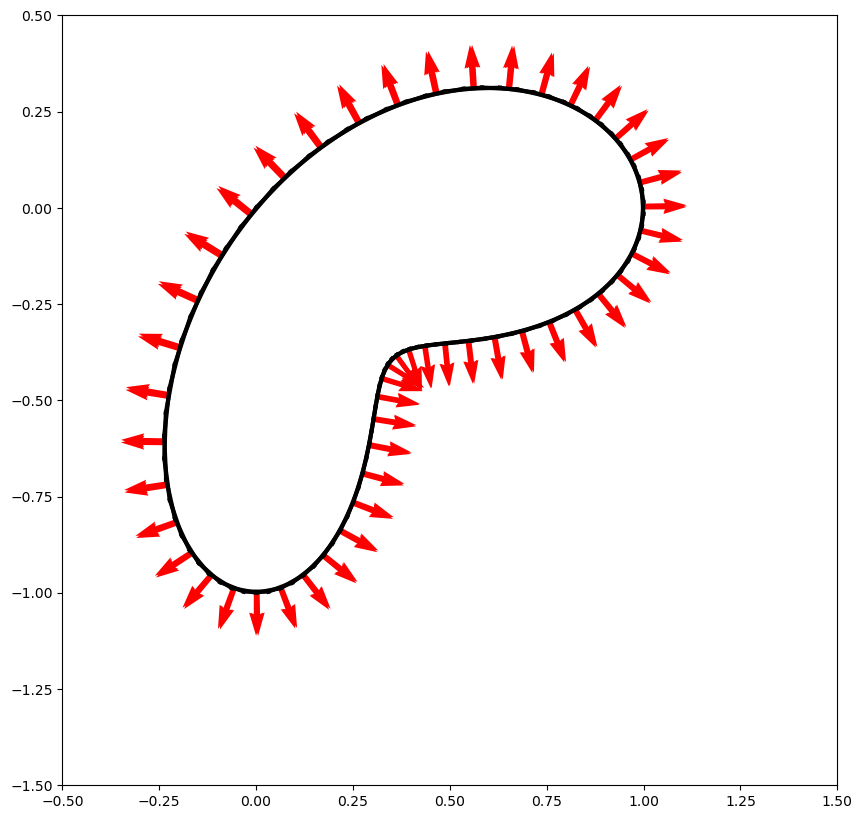
\includegraphics[width=\linewidth]{"levelset/bean/curve_bean.png"}
			\caption{"Haricot".}
		\end{figure}
	\end{minipage}
	\begin{minipage}{0.33\linewidth}
		\begin{figure}[H]
			\centering
			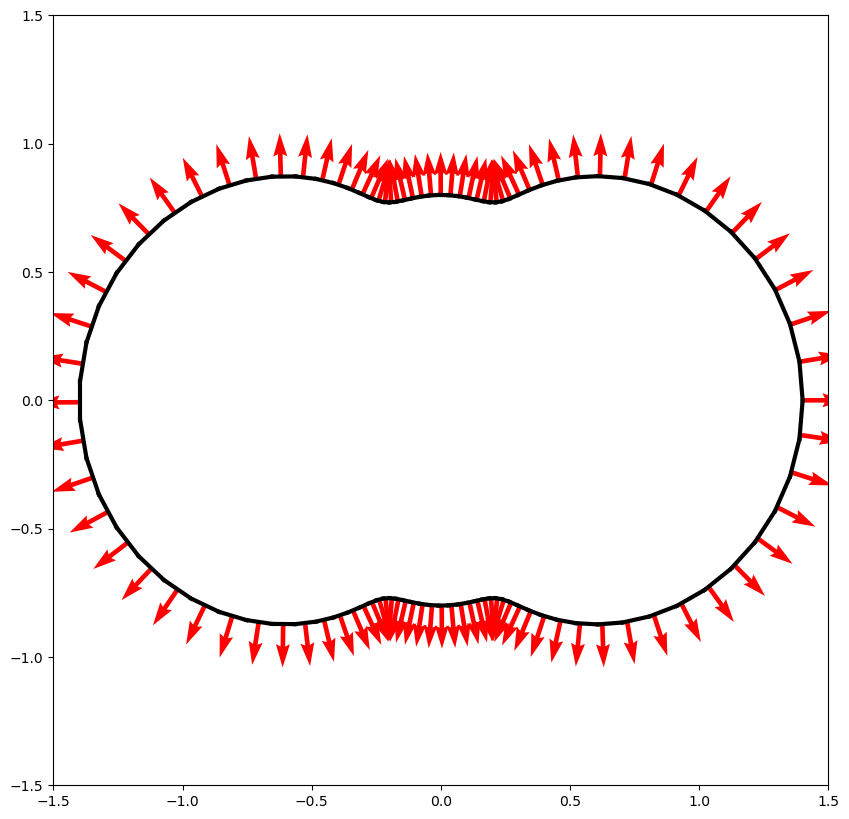
\includegraphics[width=\linewidth]{"levelset/pumpkin/curve_pumpkin.png"}
			\caption{"Citrouille".}
		\end{figure}
	\end{minipage}

	\begin{Rem}
		Ce n'est que pour une question de simplicité qu'on considère une courbe paramétrique. En pratique, on peut partir uniquement d'un ensemble de points.
	\end{Rem}

	\subsection{Trouver une levelset}
	
	Pour déterminer $\phi$, on s'est basé sur l'article \cite{CLEMOT2023368} dont l'objectif est la génération d'une distance signée par la résolution de l'équation Eikonale dans le but de générer le squelette de géométrie complexe. Comme notre objectif n'est pas le même on a du remanier ce qui était présenté dans le bus que la fonction apprise soit utilisable dans l'apprentissage d'une solution à un problème donnée. On a alors considéré les loss suivantes présentées dans l'article afin d'obtenir une solution à l'équation Eikonal :
	\begin{equation*}
		\mathcal{L}_{eik}=\int_{\mathbb{R}^2} \left(1-||\nabla \phi(p)||\right)^2 dp
	\end{equation*}
	\begin{equation*}
		\mathcal{L}_{dir}=\int_{\partial\Omega} \phi^2 dp
	\end{equation*}
	\begin{equation*}
		\mathcal{L}_{neu}=\int_{\partial\Omega} 1-\frac{n(p)\cdot\nabla\phi(p)}{||n(p)||\;||\nabla\phi(p)||} dp
	\end{equation*}

	Dans notre cas, comme l'objectif est différent, on ne cherchera pas à approcher la sdf de la géométrie, on souhaite en fait déterminer une fonction levelset qui a certaines bonnes propriétés qui permettraient de l'utiliser par la suite. En particulier, on cherchera à limiter l'explosion des dérivées secondes et pour cela, on ajoutera la loss suivante : 
	\begin{equation*}
		\mathcal{L}_{lap}=\int_{\mathbb{R}^2} \Delta\phi^2 dp
	\end{equation*}

	Pour la résolution du problème, on considérera un PINNs dont le modèle sera défini par un simple MLP et on cherchera $\phi_\theta(x,y)$ avec la loss définie par
	\begin{equation*}
		\mathcal{L}=w_{eik}\mathcal{L}_{eik}+w_{dir}\mathcal{L}_{dir}+w_{neu}\mathcal{L}_{neu}+w_{lap}\mathcal{L}_{lap}
	\end{equation*}
	
	\begin{Rem}
		Pour l'instant, on entraîne un modèle par géométrie mais dans la suite on cherchera à construire un modèle paramétrique.
	\end{Rem}

	\subsection{Résultats}
	
	\textbf{Circle :}
	
	\begin{figure}[H]
		\centering
		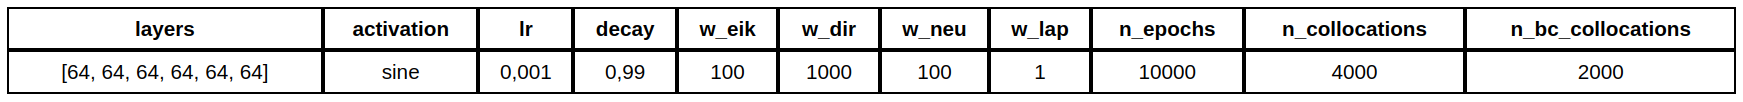
\includegraphics[width=\linewidth]{"levelset/circle/config_circle.png"}
		\caption{Configuration.}
	\end{figure}
	
	\begin{minipage}{0.33\linewidth}
		\begin{figure}[H]
			\centering
			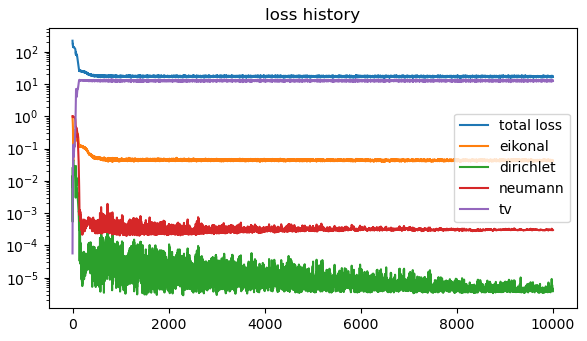
\includegraphics[width=\linewidth]{"levelset/circle/loss_circle.png"}
			\caption{Loss (tv=lap).}
		\end{figure}
	\end{minipage}
	\begin{minipage}{0.33\linewidth}
		\begin{figure}[H]
			\centering
			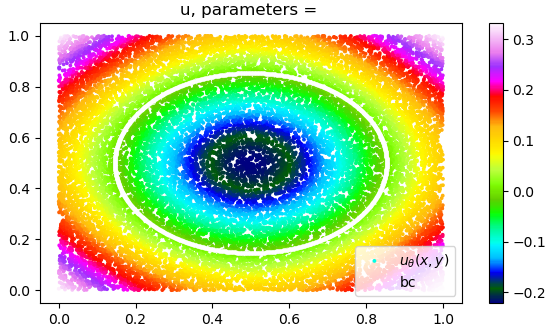
\includegraphics[width=\linewidth]{"levelset/circle/sol_circle.png"}
			\caption{Levelset $\phi_\theta$.}
		\end{figure}
	\end{minipage}
	\begin{minipage}{0.33\linewidth}
		\begin{figure}[H]
			\centering
			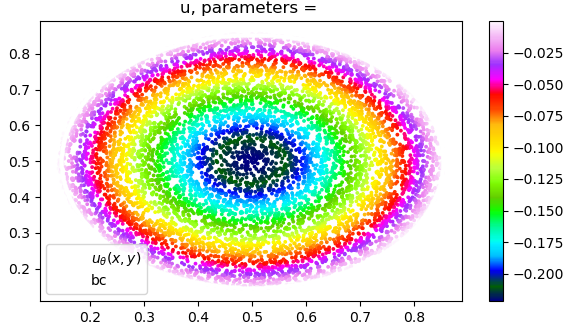
\includegraphics[width=\linewidth]{"levelset/circle/sol_mask_circle.png"}
			\caption{Levelset $\phi_\theta<0$.}
		\end{figure}
	\end{minipage}

	\begin{minipage}{0.56\linewidth}
		\begin{figure}[H]
			\centering
			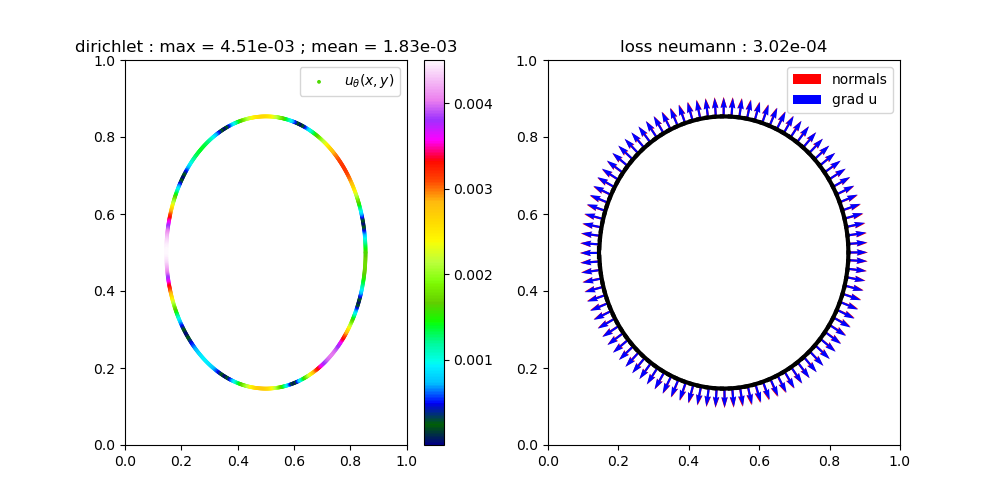
\includegraphics[width=\linewidth]{"levelset/circle/bc_circle.png"}
			\caption{Loss (tv=lap).}
		\end{figure}
	\end{minipage}
	\begin{minipage}{0.43\linewidth}
		\begin{figure}[H]
			\centering
			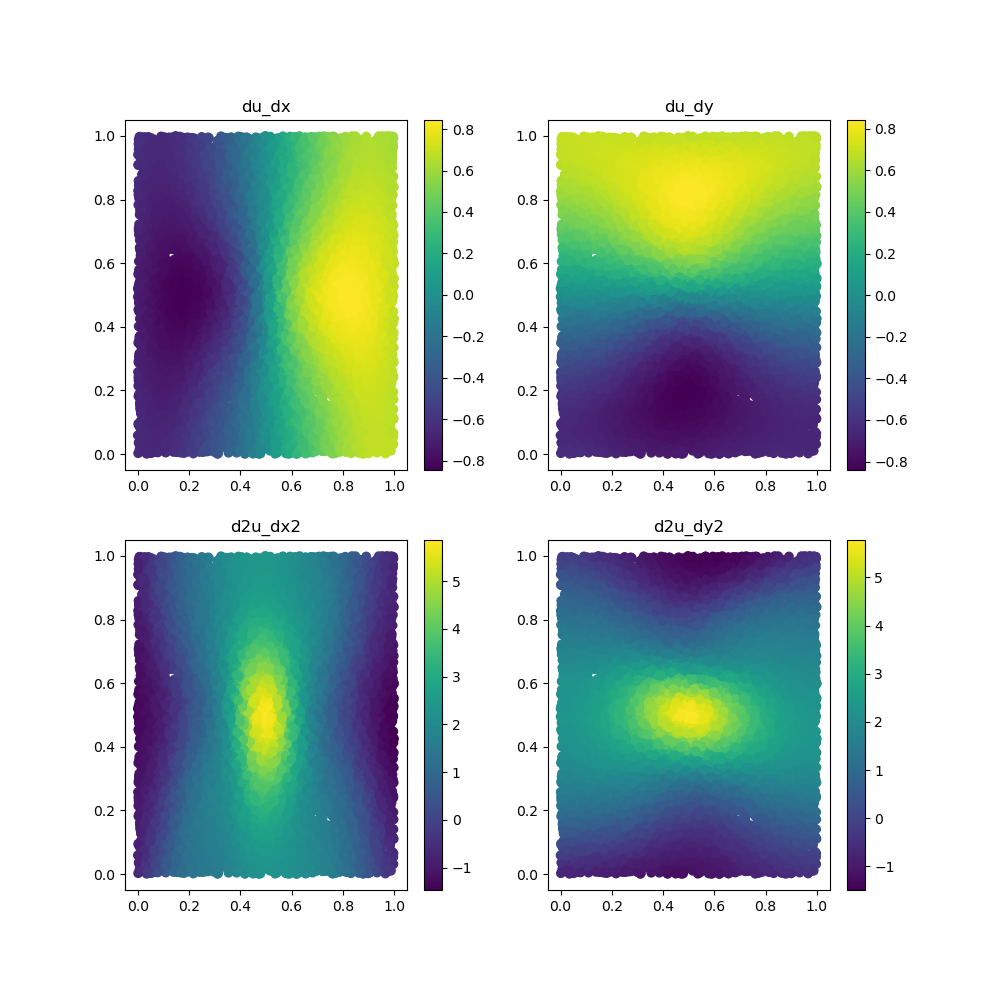
\includegraphics[width=\linewidth]{"levelset/circle/derivees_circle.png"}
			\caption{Levelset $\phi_\theta$.}
		\end{figure}
	\end{minipage}
	
	\newpage
	\textbf{Bean :}
	
	\begin{figure}[H]
		\centering
		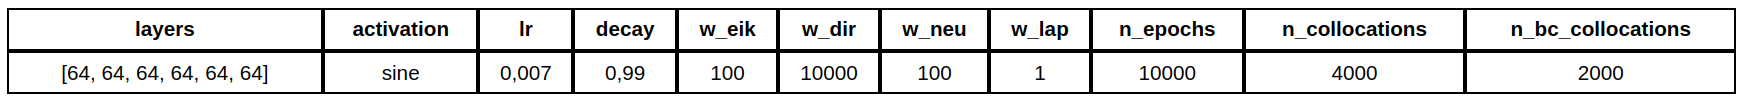
\includegraphics[width=\linewidth]{"levelset/bean/config_bean.png"}
		\caption{Configuration.}
	\end{figure}
	
	\begin{minipage}{0.33\linewidth}
		\begin{figure}[H]
			\centering
			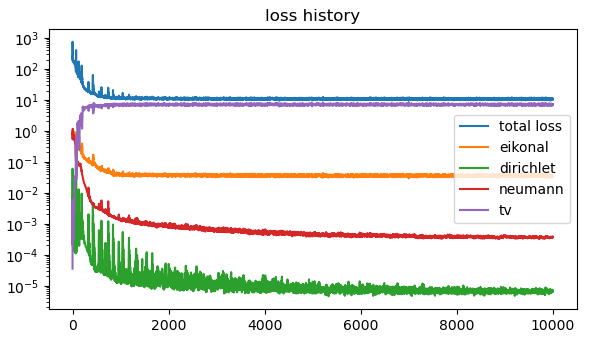
\includegraphics[width=\linewidth]{"levelset/bean/loss_bean.png"}
			\caption{Loss (tv=lap).}
		\end{figure}
	\end{minipage}
	\begin{minipage}{0.33\linewidth}
		\begin{figure}[H]
			\centering
			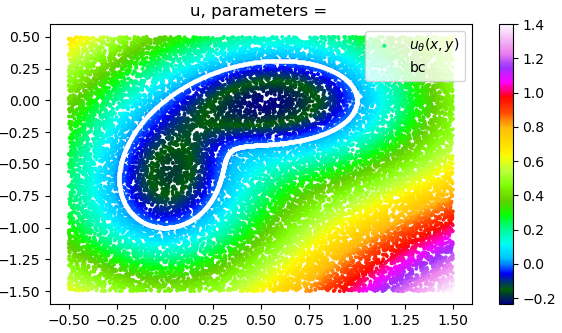
\includegraphics[width=\linewidth]{"levelset/bean/sol_bean.png"}
			\caption{Levelset $\phi_\theta$.}
		\end{figure}
	\end{minipage}
	\begin{minipage}{0.33\linewidth}
		\begin{figure}[H]
			\centering
			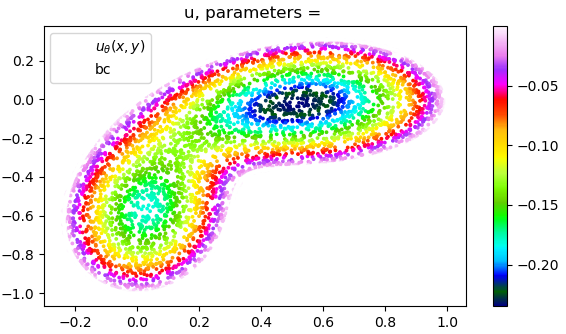
\includegraphics[width=\linewidth]{"levelset/bean/sol_mask_bean.png"}
			\caption{Levelset $\phi_\theta<0$.}
		\end{figure}
	\end{minipage}
	
	\begin{minipage}{0.56\linewidth}
		\begin{figure}[H]
			\centering
			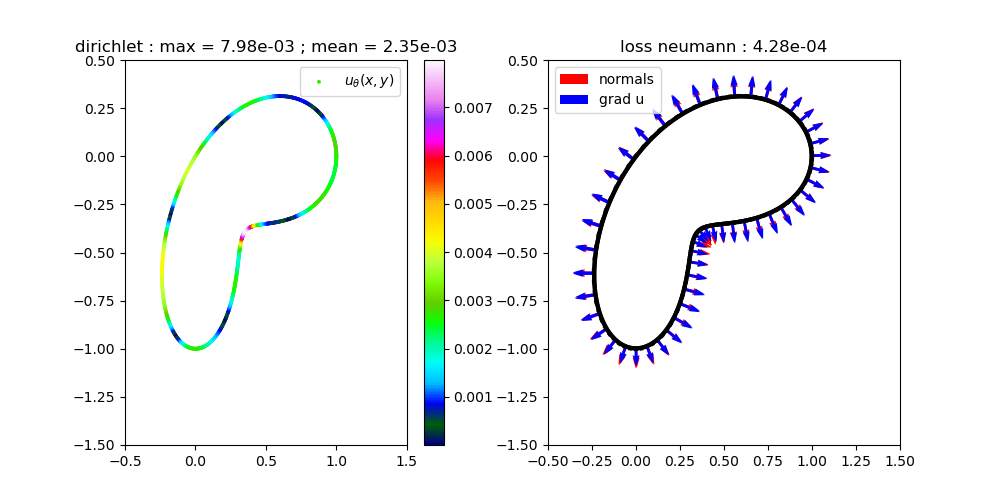
\includegraphics[width=\linewidth]{"levelset/bean/bc_bean.png"}
			\caption{Loss (tv=lap).}
		\end{figure}
	\end{minipage}
	\begin{minipage}{0.43\linewidth}
		\begin{figure}[H]
			\centering
			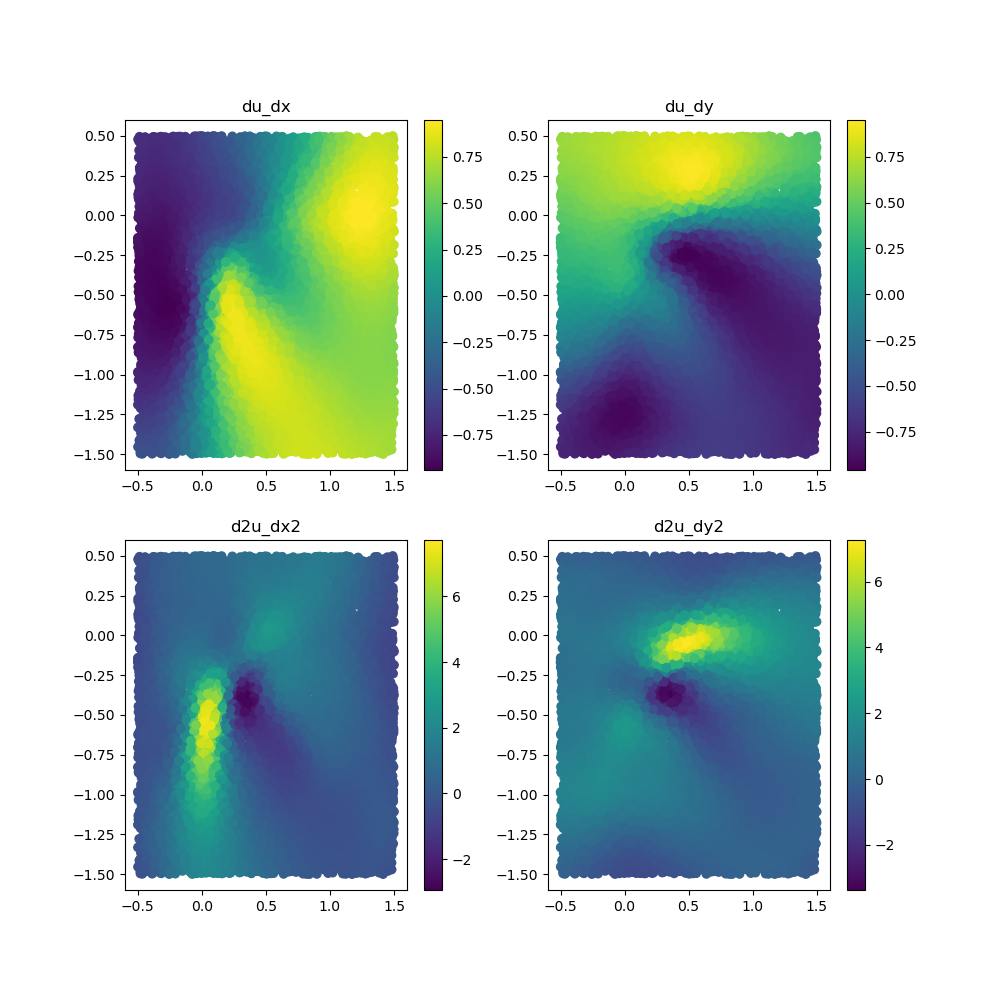
\includegraphics[width=\linewidth]{"levelset/bean/derivees_bean.png"}
			\caption{Levelset $\phi_\theta$.}
		\end{figure}
	\end{minipage}

	\textbf{Pumpkin :}
	
	\begin{figure}[H]
		\centering
		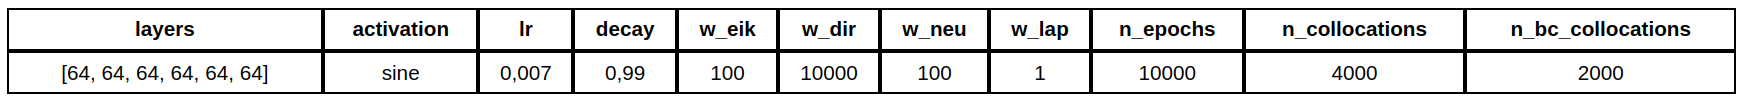
\includegraphics[width=\linewidth]{"levelset/pumpkin/config_pumpkin.png"}
		\caption{Configuration.}
	\end{figure}
	
	\begin{minipage}{0.33\linewidth}
		\begin{figure}[H]
			\centering
			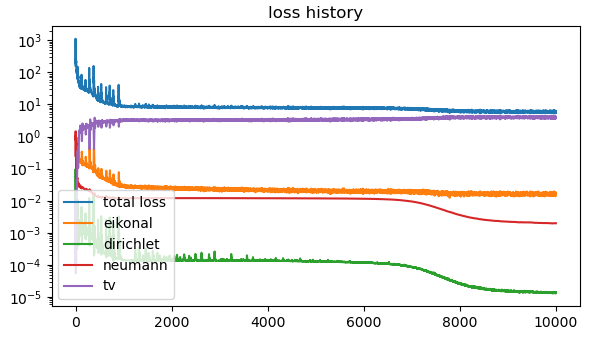
\includegraphics[width=\linewidth]{"levelset/pumpkin/loss_pumpkin.png"}
			\caption{Loss (tv=lap).}
		\end{figure}
	\end{minipage}
	\begin{minipage}{0.33\linewidth}
		\begin{figure}[H]
			\centering
			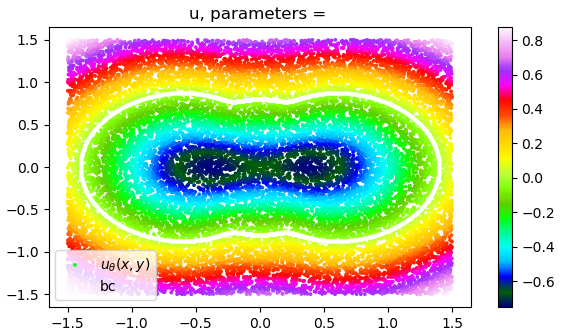
\includegraphics[width=\linewidth]{"levelset/pumpkin/sol_pumpkin.png"}
			\caption{Levelset $\phi_\theta$.}
		\end{figure}
	\end{minipage}
	\begin{minipage}{0.33\linewidth}
		\begin{figure}[H]
			\centering
			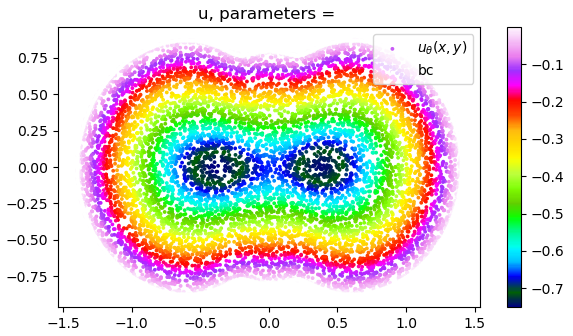
\includegraphics[width=\linewidth]{"levelset/pumpkin/sol_mask_pumpkin.png"}
			\caption{Levelset $\phi_\theta<0$.}
		\end{figure}
	\end{minipage}
	
	\begin{minipage}{0.56\linewidth}
		\begin{figure}[H]
			\centering
			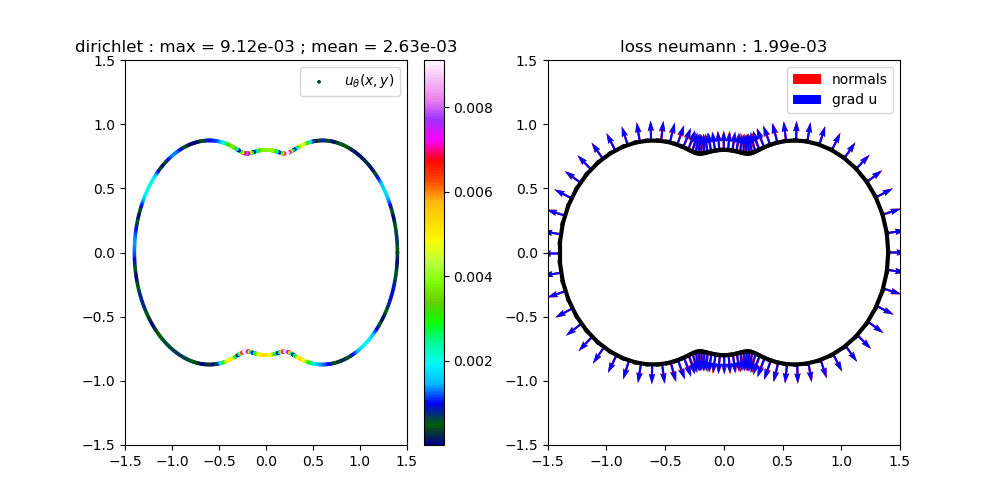
\includegraphics[width=\linewidth]{"levelset/pumpkin/bc_pumpkin.png"}
			\caption{Loss (tv=lap).}
		\end{figure}
	\end{minipage}
	\begin{minipage}{0.43\linewidth}
		\begin{figure}[H]
			\centering
			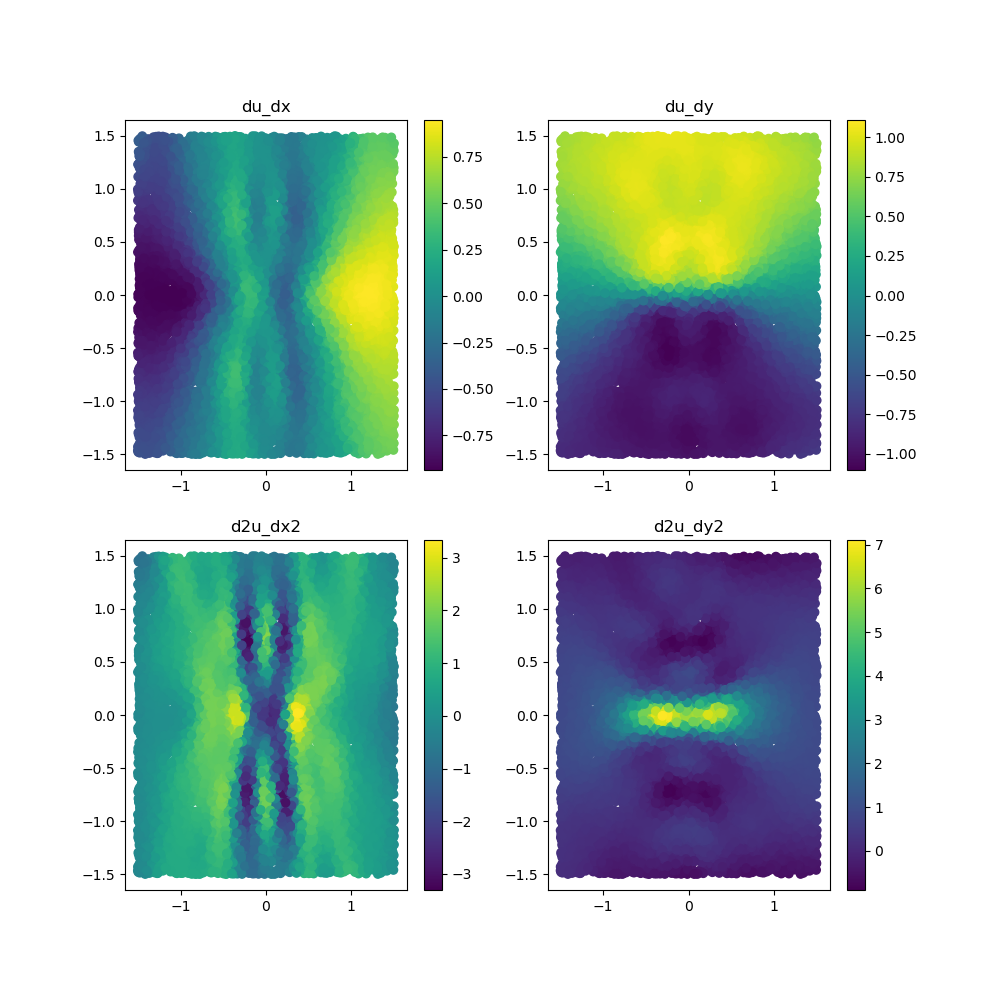
\includegraphics[width=\linewidth]{"levelset/pumpkin/derivees_pumpkin.png"}
			\caption{Levelset $\phi_\theta$.}
		\end{figure}
	\end{minipage}

	\section{Étape 2 : Résolution de Poisson}
	
	On considère le problème suivant
	\begin{equation*}
		\left\{\begin{aligned}
			&-\Delta u=1 \; \text{dans } \Omega \\
			&u=0 \; \text{sur } \partial\Omega
		\end{aligned}\right.
	\end{equation*}
	où $\Omega$ pourra représenter le cercle, le haricot ou la citrouille.
	
	On cherchera à entraîner un nouveau PINNs à apprendre $w$ tel que $u=\phi_\theta w$ avec $\phi_ \theta$ la levelset apprise précédemment.
	
	\textbf{Circle :}
	
	\begin{figure}[H]
		\centering
		\includegraphics[width=\linewidth]{"poisson/circle/config.png"}
		\caption{Configuration.}
	\end{figure}
	
	\begin{minipage}{0.48\linewidth}
		\begin{figure}[H]
			\centering
			\includegraphics[width=0.9\linewidth]{"poisson/circle/loss.png"}
			\caption{Loss.}
		\end{figure}
	\end{minipage}
	\begin{minipage}{0.48\linewidth}
		\begin{figure}[H]
			\centering
			\includegraphics[width=0.9\linewidth]{"poisson/circle/sol.png"}
			\caption{Sol $u_\theta$.}
		\end{figure}
	\end{minipage}
	
	\begin{figure}[H]
			\centering
			\includegraphics[width=\linewidth]{"poisson/circle/compare.png"}
			\caption{Comparaison avec une solution FEM sur-rafinée.}
	\end{figure}

	\textbf{Bean - 1 :}
	
	\begin{figure}[H]
		\centering
		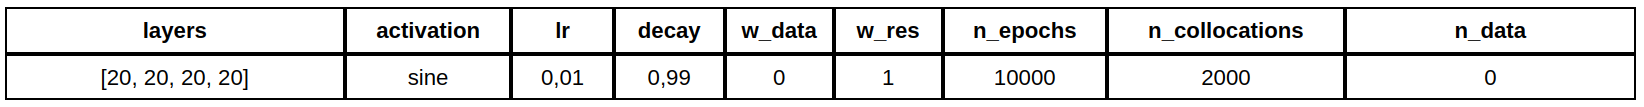
\includegraphics[width=\linewidth]{"poisson/bean/config_1.png"}
		\caption{Configuration.}
	\end{figure}
	
	\begin{minipage}{0.48\linewidth}
		\begin{figure}[H]
			\centering
			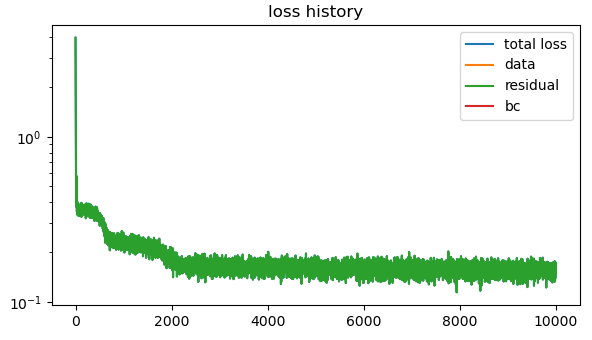
\includegraphics[width=0.9\linewidth]{"poisson/bean/loss_1.png"}
			\caption{Loss.}
		\end{figure}
	\end{minipage}
	\begin{minipage}{0.48\linewidth}
		\begin{figure}[H]
			\centering
			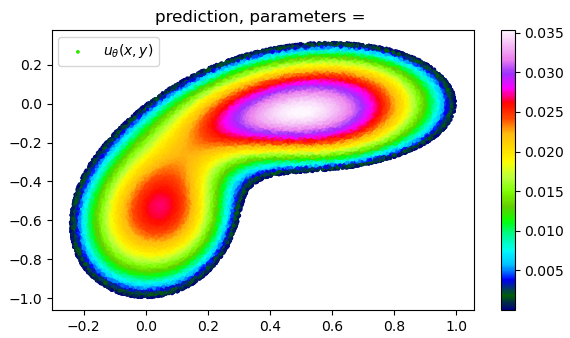
\includegraphics[width=0.9\linewidth]{"poisson/bean/sol_1.png"}
			\caption{Sol $u_\theta$.}
		\end{figure}
	\end{minipage}
	
	\begin{figure}[H]
		\centering
		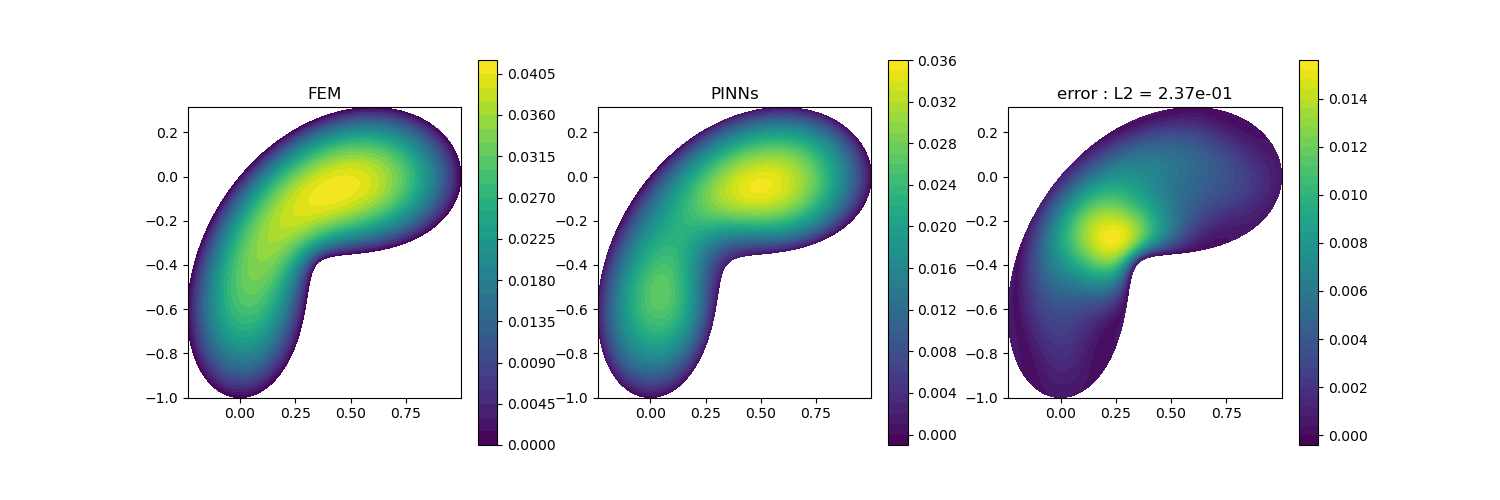
\includegraphics[width=\linewidth]{"poisson/bean/compare_1.png"}
		\caption{Comparaison avec une solution FEM sur-rafinée.}
	\end{figure}

	\newpage

	\textbf{Bean - 2 :}
	
	\begin{figure}[H]
		\centering
		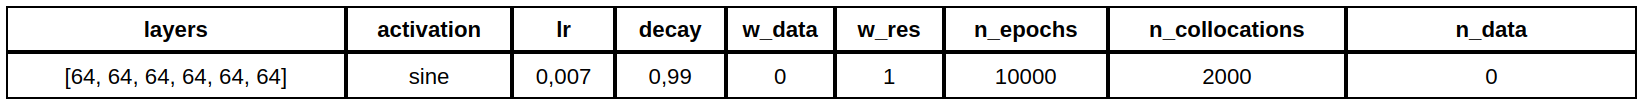
\includegraphics[width=\linewidth]{"poisson/bean/config_2.png"}
		\caption{Configuration.}
	\end{figure}
	
	\begin{minipage}{0.48\linewidth}
		\begin{figure}[H]
			\centering
			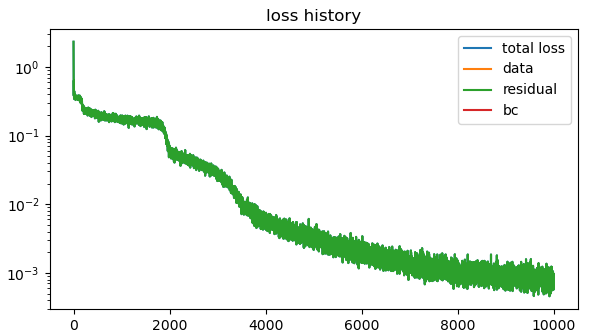
\includegraphics[width=0.9\linewidth]{"poisson/bean/loss_2.png"}
			\caption{Loss.}
		\end{figure}
	\end{minipage}
	\begin{minipage}{0.48\linewidth}
		\begin{figure}[H]
			\centering
			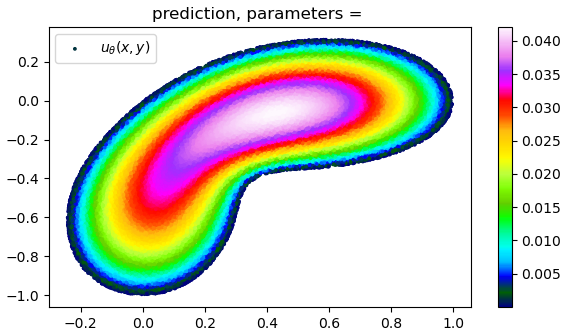
\includegraphics[width=0.9\linewidth]{"poisson/bean/sol_2.png"}
			\caption{Sol $u_\theta$.}
		\end{figure}
	\end{minipage}
	
	\begin{figure}[H]
		\centering
		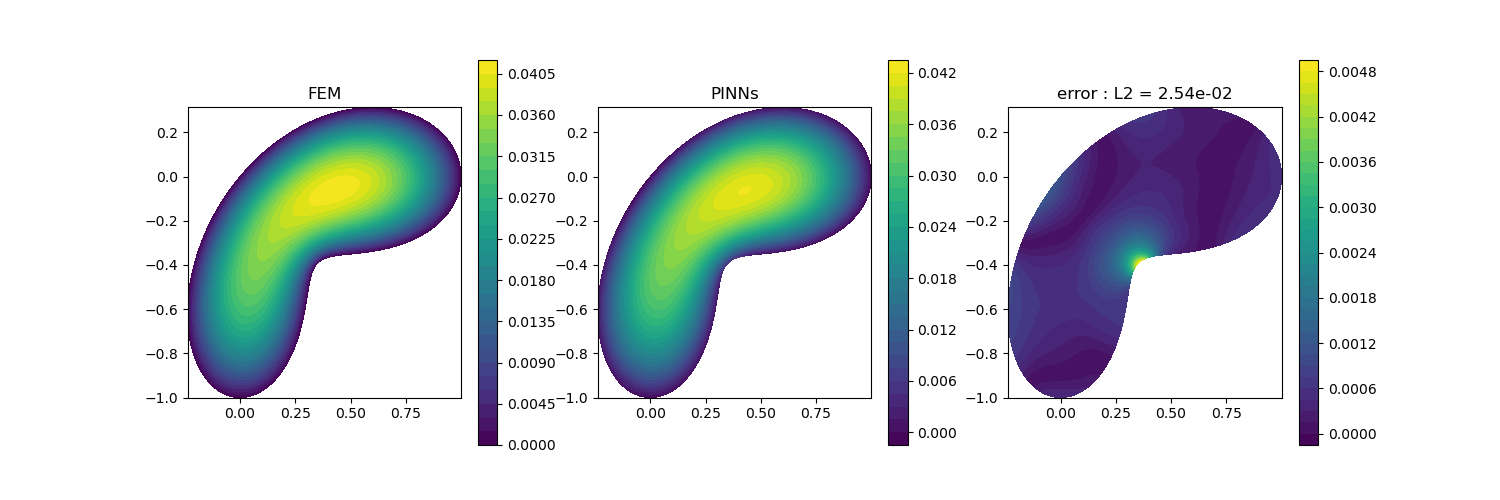
\includegraphics[width=\linewidth]{"poisson/bean/compare_2.png"}
		\caption{Comparaison avec une solution FEM sur-rafinée.}
	\end{figure}
	
	\textbf{Pumpkin :}
	
	\begin{figure}[H]
		\centering
		\includegraphics[width=\linewidth]{"poisson/pumpkin/config.png"}
		\caption{Configuration.}
	\end{figure}
	
	\begin{minipage}{0.48\linewidth}
		\begin{figure}[H]
			\centering
			\includegraphics[width=0.9\linewidth]{"poisson/pumpkin/loss.png"}
			\caption{Loss.}
		\end{figure}
	\end{minipage}
	\begin{minipage}{0.48\linewidth}
		\begin{figure}[H]
			\centering
			\includegraphics[width=0.9\linewidth]{"poisson/pumpkin/sol.png"}
			\caption{Sol $u_\theta$.}
		\end{figure}
	\end{minipage}
	
	\begin{figure}[H]
		\centering
		\includegraphics[width=\linewidth]{"poisson/pumpkin/compare.png"}
		\caption{Comparaison avec une solution FEM sur-rafinée.}
	\end{figure}

	\newpage
	\section{Étape 3 : Correction par addition}
	
	\subsection{Avec FEM}
	
	\textbf{Circle :}
	
	\begin{figure}[H]
		\centering
		\includegraphics[width=0.55\linewidth]{"correction/circle/corr_FEM.png"}
		\caption{Correction par addition avec FEM.}
	\end{figure}
	
	\textbf{Bean - 1 :}
	
	\begin{figure}[H]
		\centering
		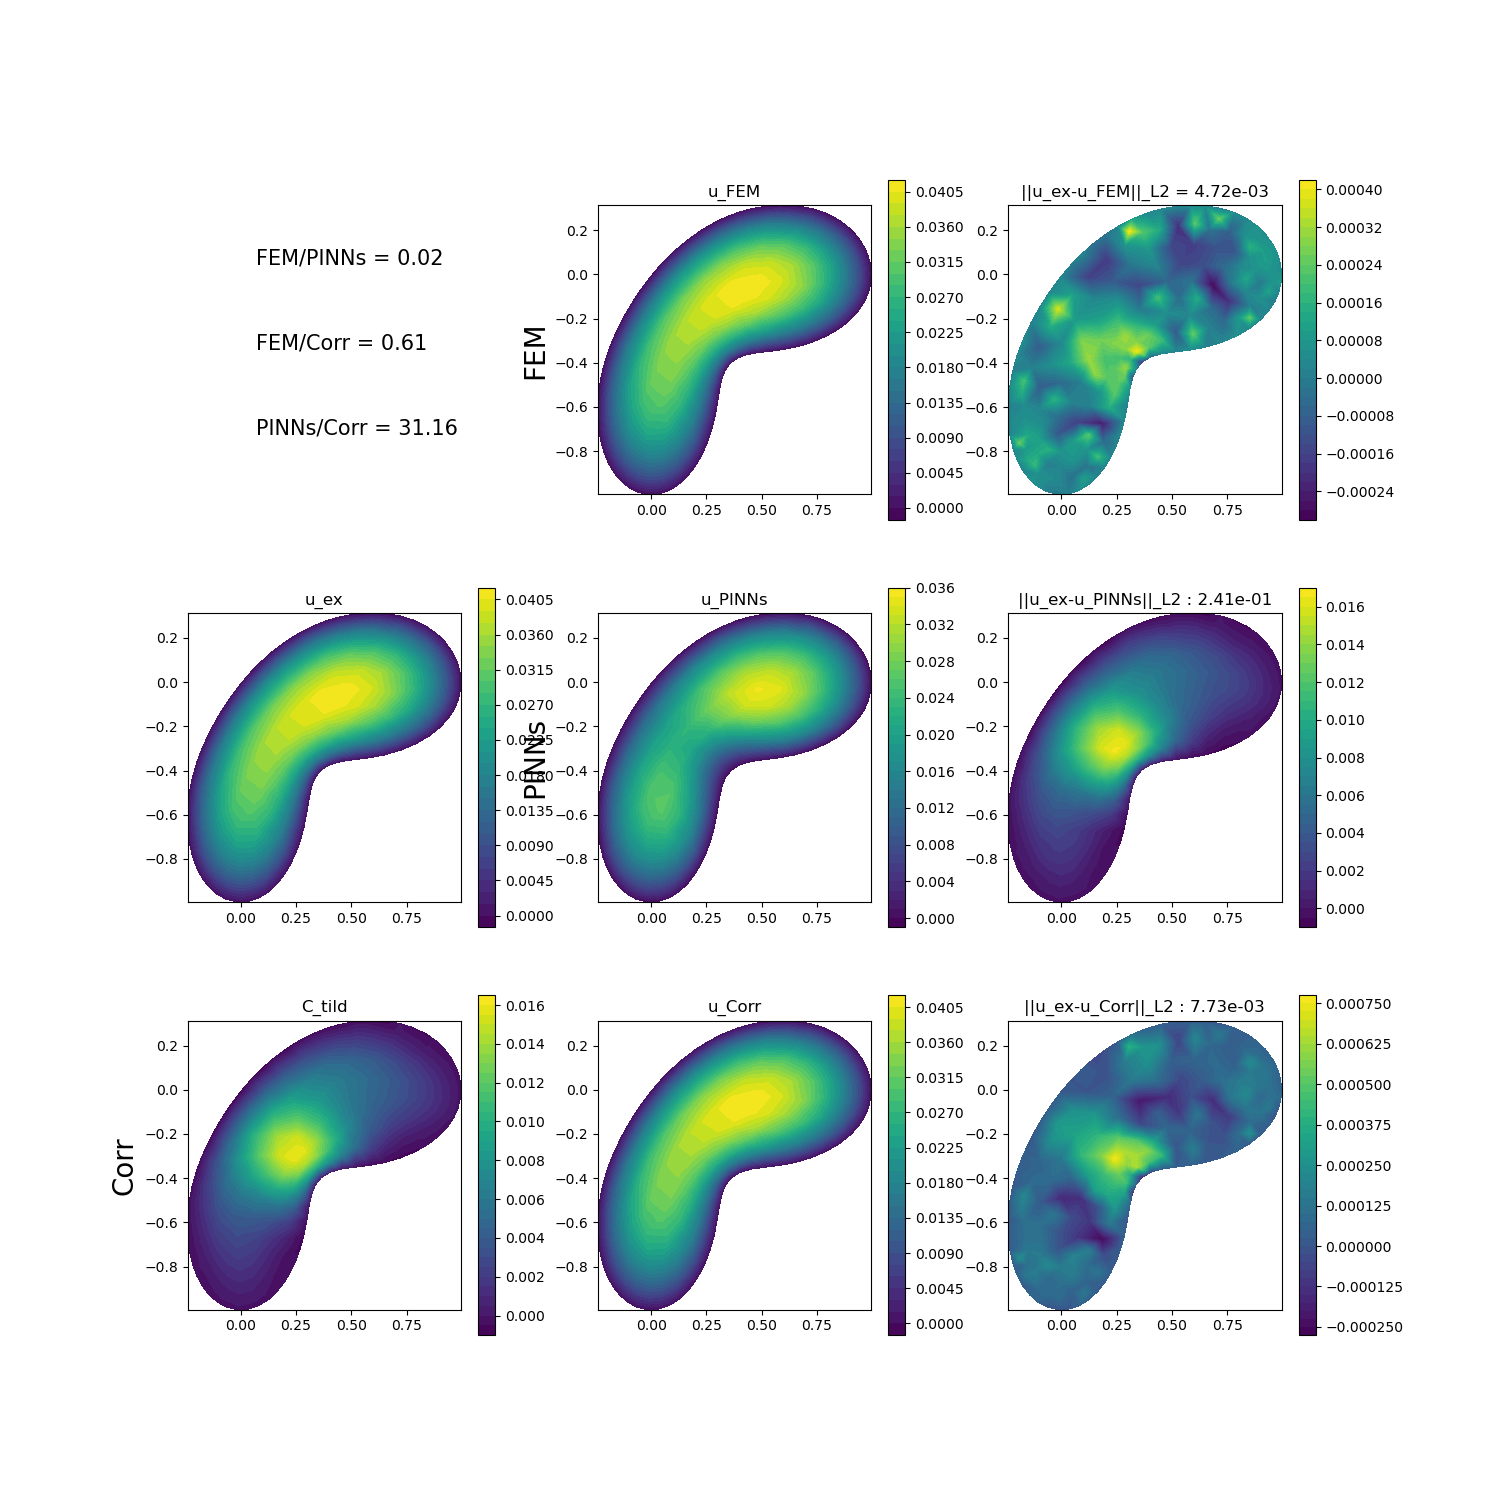
\includegraphics[width=0.55\linewidth]{"correction/bean/corr_FEM_1.png"}
		\caption{Correction par addition avec FEM.}
	\end{figure}

	\textbf{Bean - 2 :}
	
	\begin{figure}[H]
		\centering
		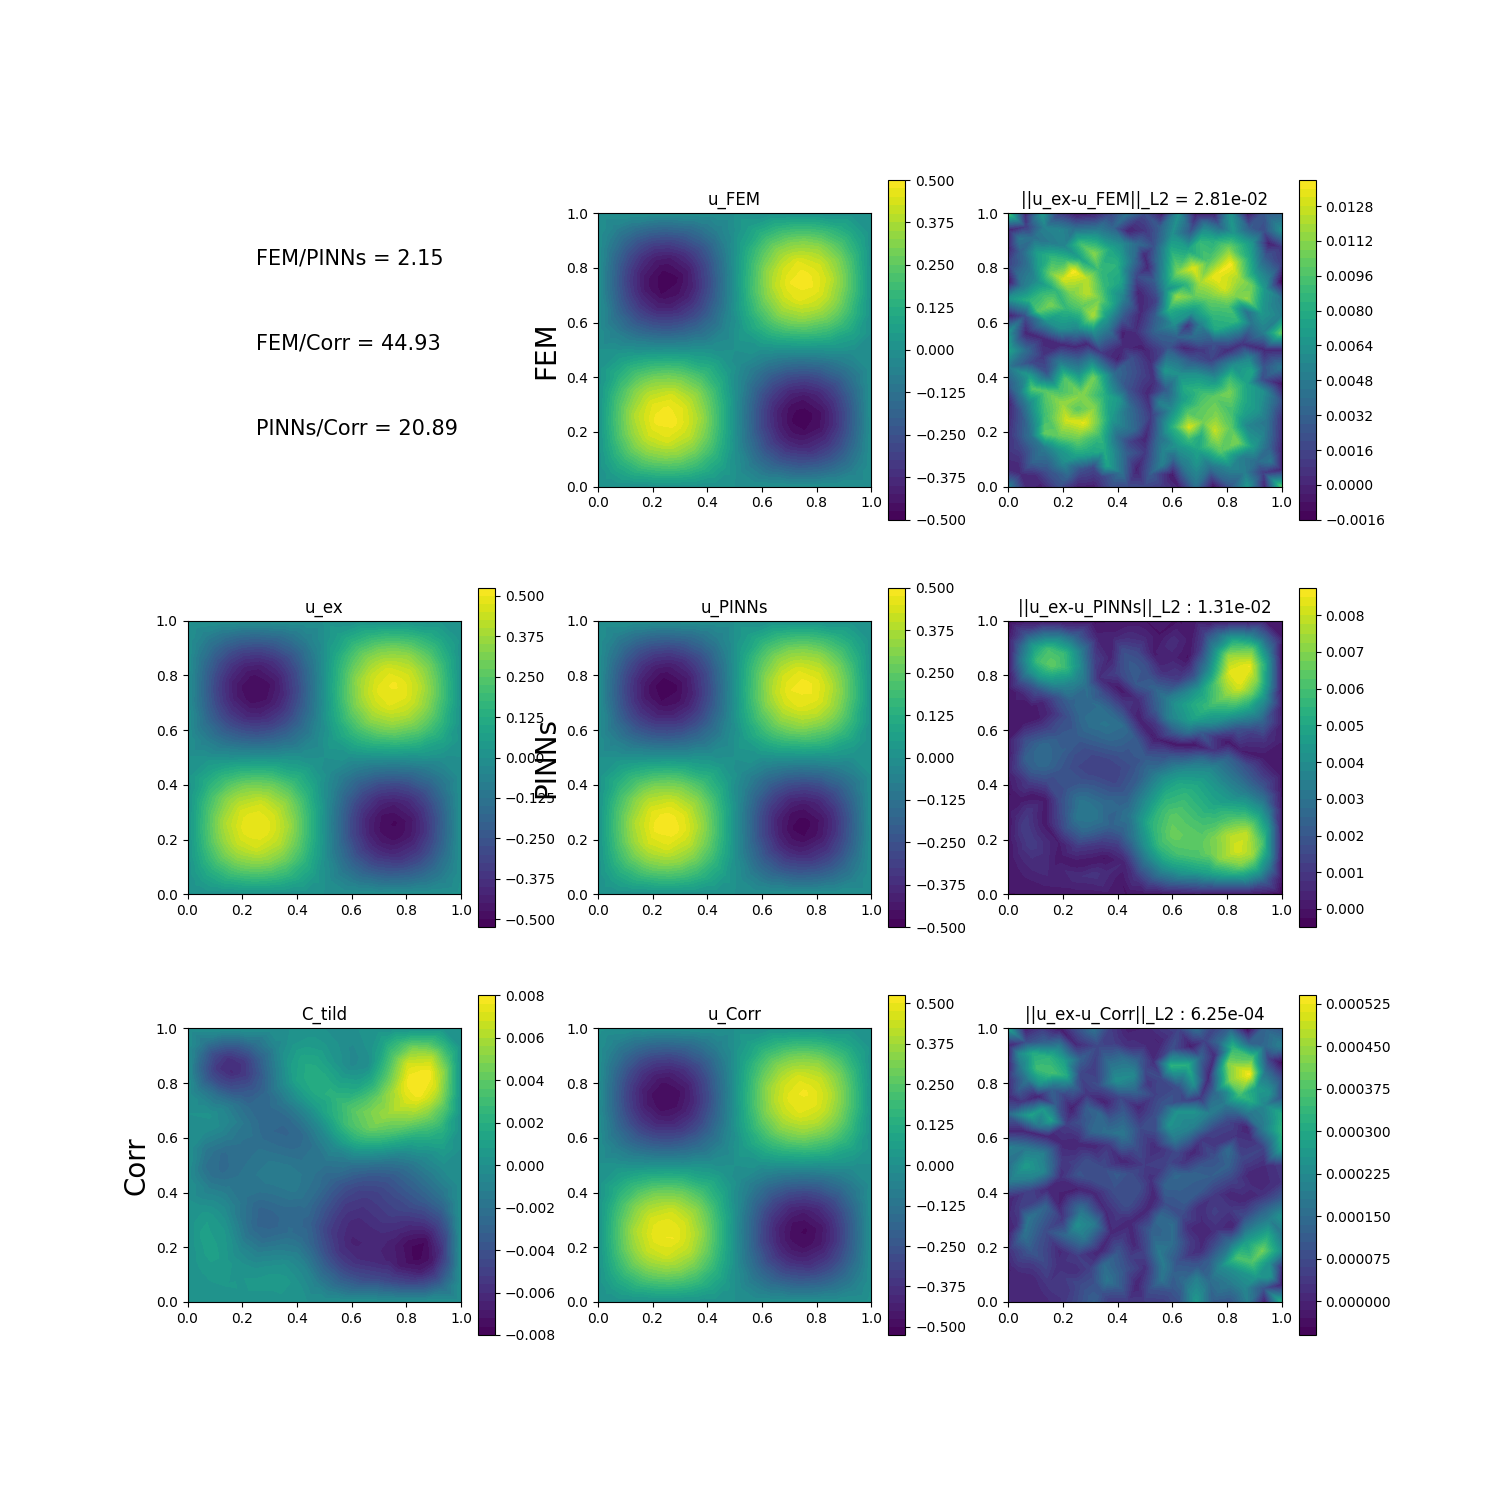
\includegraphics[width=0.55\linewidth]{"correction/bean/corr_FEM_2.png"}
		\caption{Correction par addition avec FEM.}
	\end{figure}

	\textbf{Pumpkin :}
	
	\begin{figure}[H]
		\centering
		\includegraphics[width=0.55\linewidth]{"correction/pumpkin/corr_FEM.png"}
		\caption{Correction par addition avec FEM.}
	\end{figure}
	
	
	\newpage
	\subsection{Avec $\phi$-FEM}
	
	\textbf{Circle :}
	
	\begin{figure}[H]
		\centering
		\includegraphics[width=0.6\linewidth]{"correction/circle/corr_PhiFEM.png"}
		\caption{Correction par addition avec $\phi$-FEM.}
	\end{figure}

	\begin{figure}[H]
		\centering
		\includegraphics[width=0.6\linewidth]{"correction/circle/corr_PhiFEM_Omega.png"}
		\caption{Correction par addition avec $\phi$-FEM (projeté).}
	\end{figure}
	
	\newpage
	\textbf{Bean - 1 :}
	
	\begin{figure}[H]
		\centering
		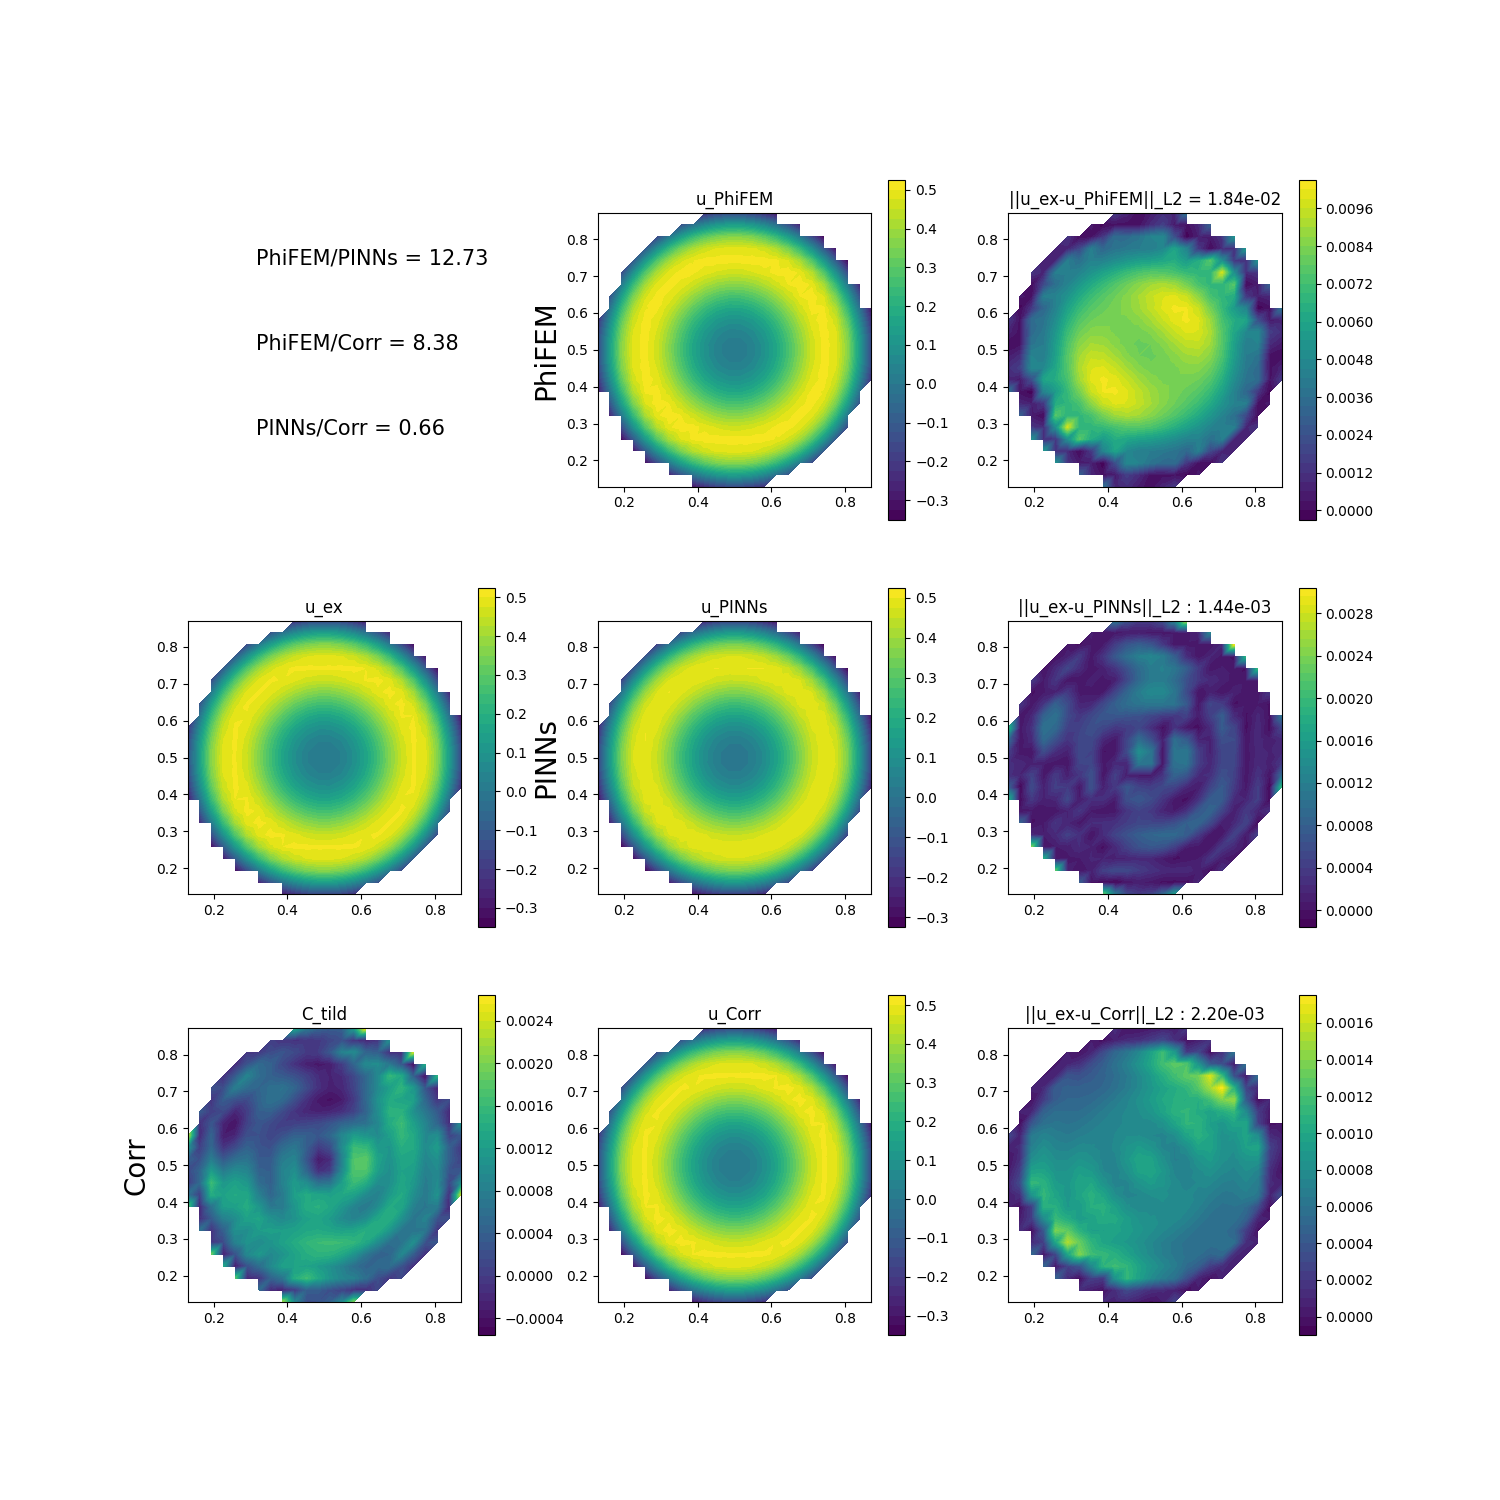
\includegraphics[width=0.6\linewidth]{"correction/bean/corr_PhiFEM_1.png"}
		\caption{Correction par addition avec $\phi$-FEM.}
	\end{figure}
	
	\begin{figure}[H]
		\centering
		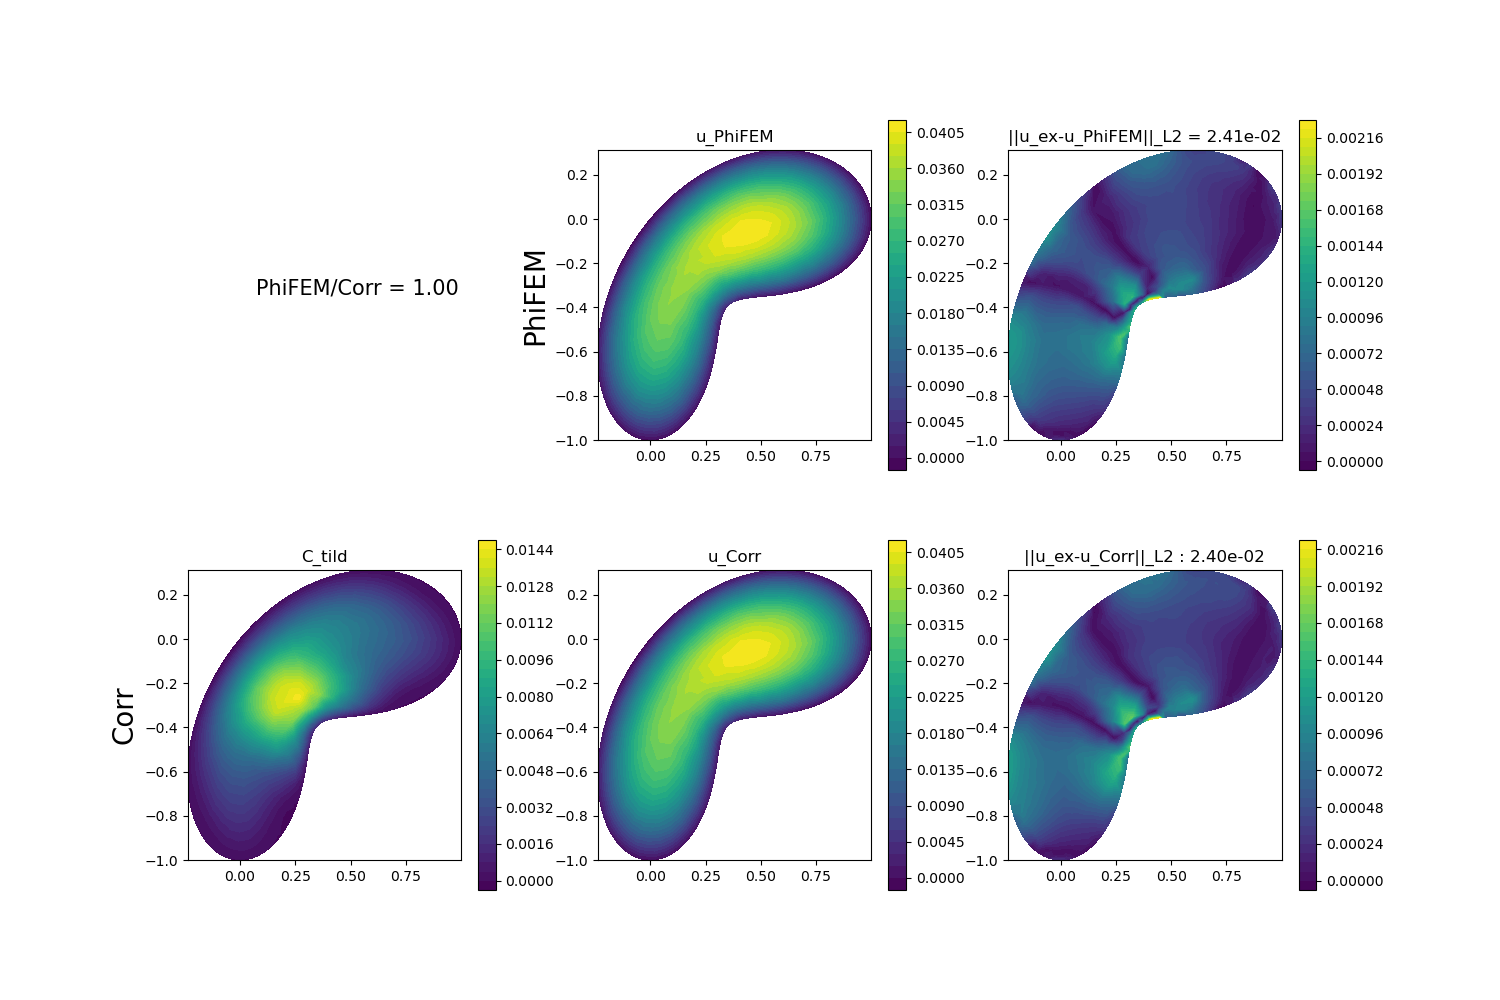
\includegraphics[width=0.6\linewidth]{"correction/bean/corr_PhiFEM_1_Omega.png"}
		\caption{Correction par addition avec $\phi$-FEM (projeté).}
	\end{figure}

	\newpage
	\textbf{Bean - 2 :}
	
	\begin{figure}[H]
		\centering
		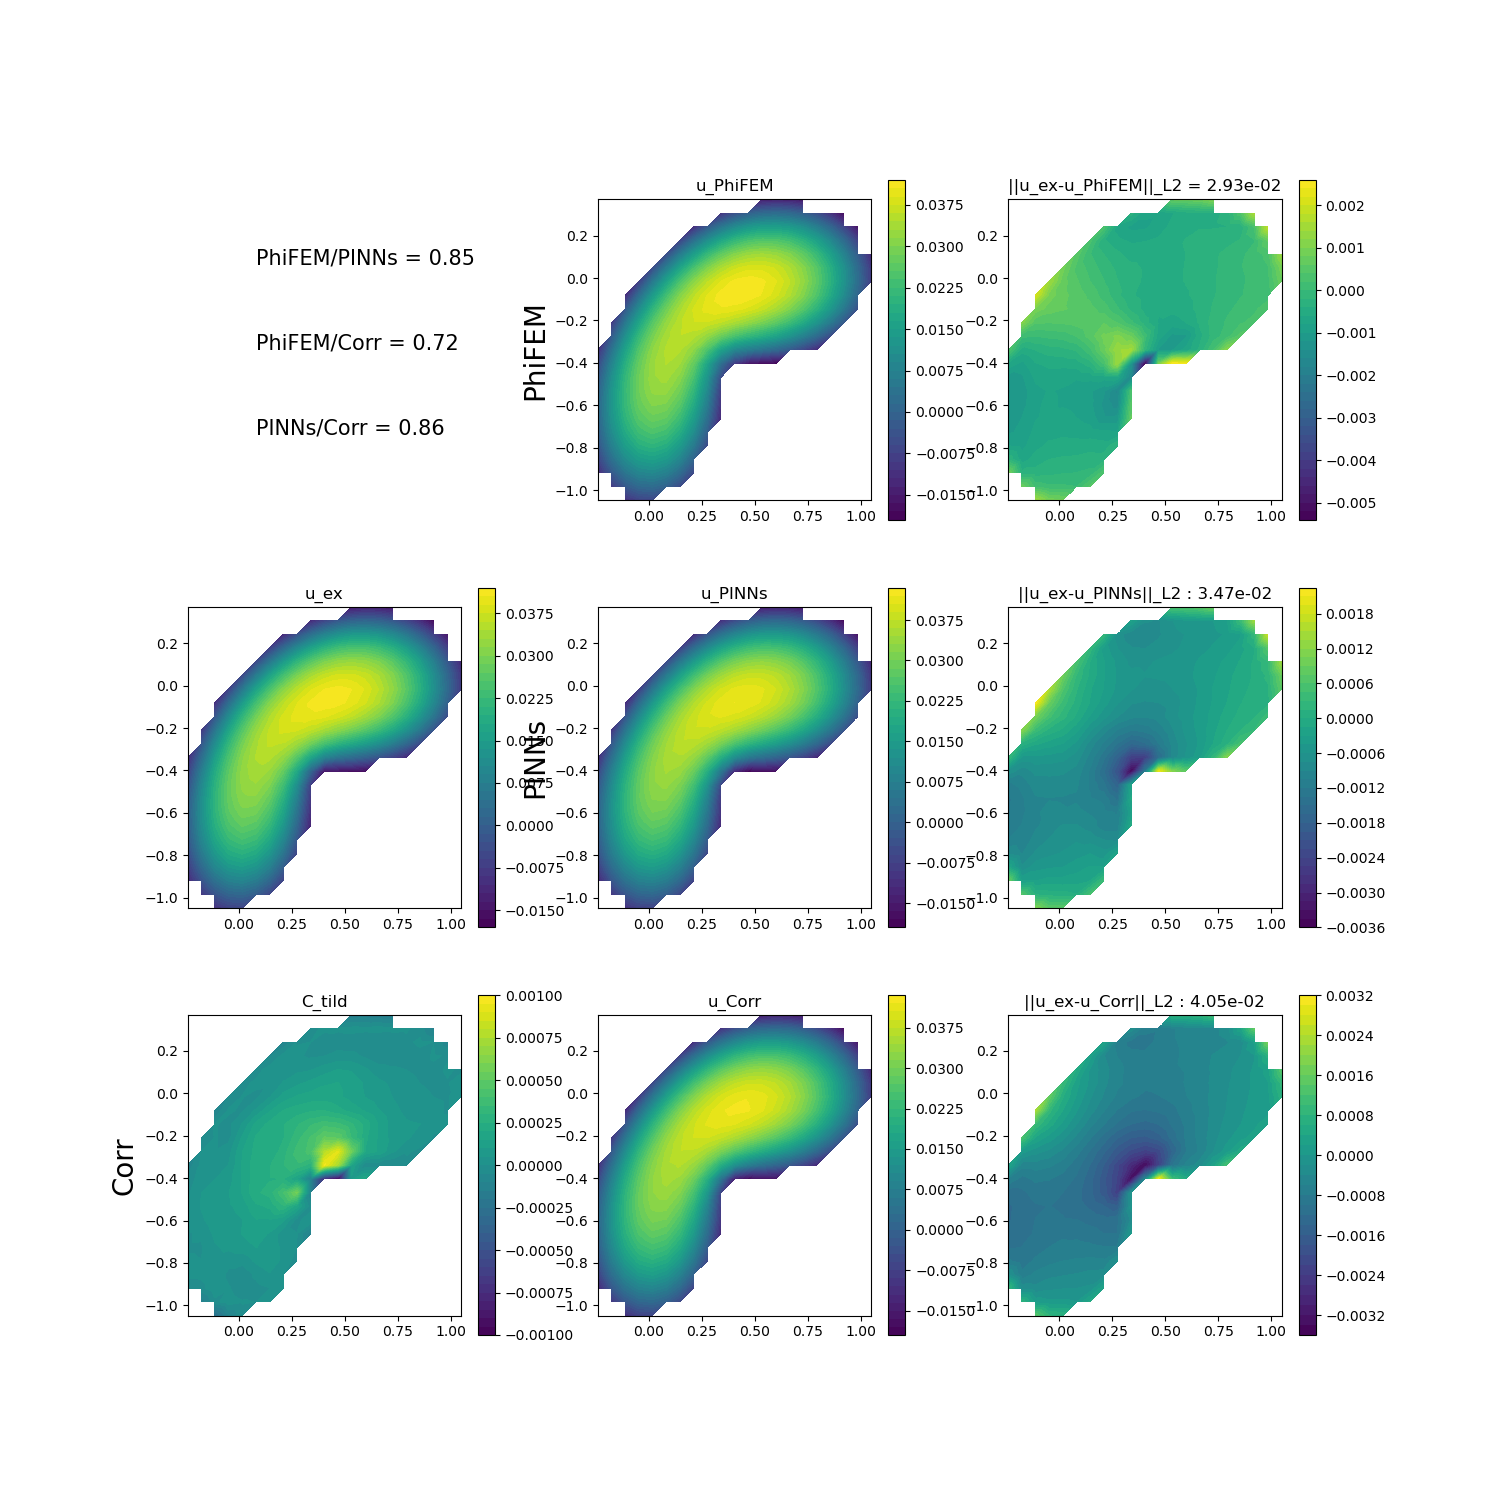
\includegraphics[width=0.6\linewidth]{"correction/bean/corr_PhiFEM_2.png"}
		\caption{Correction par addition avec $\phi$-FEM.}
	\end{figure}
	
	\begin{figure}[H]
		\centering
		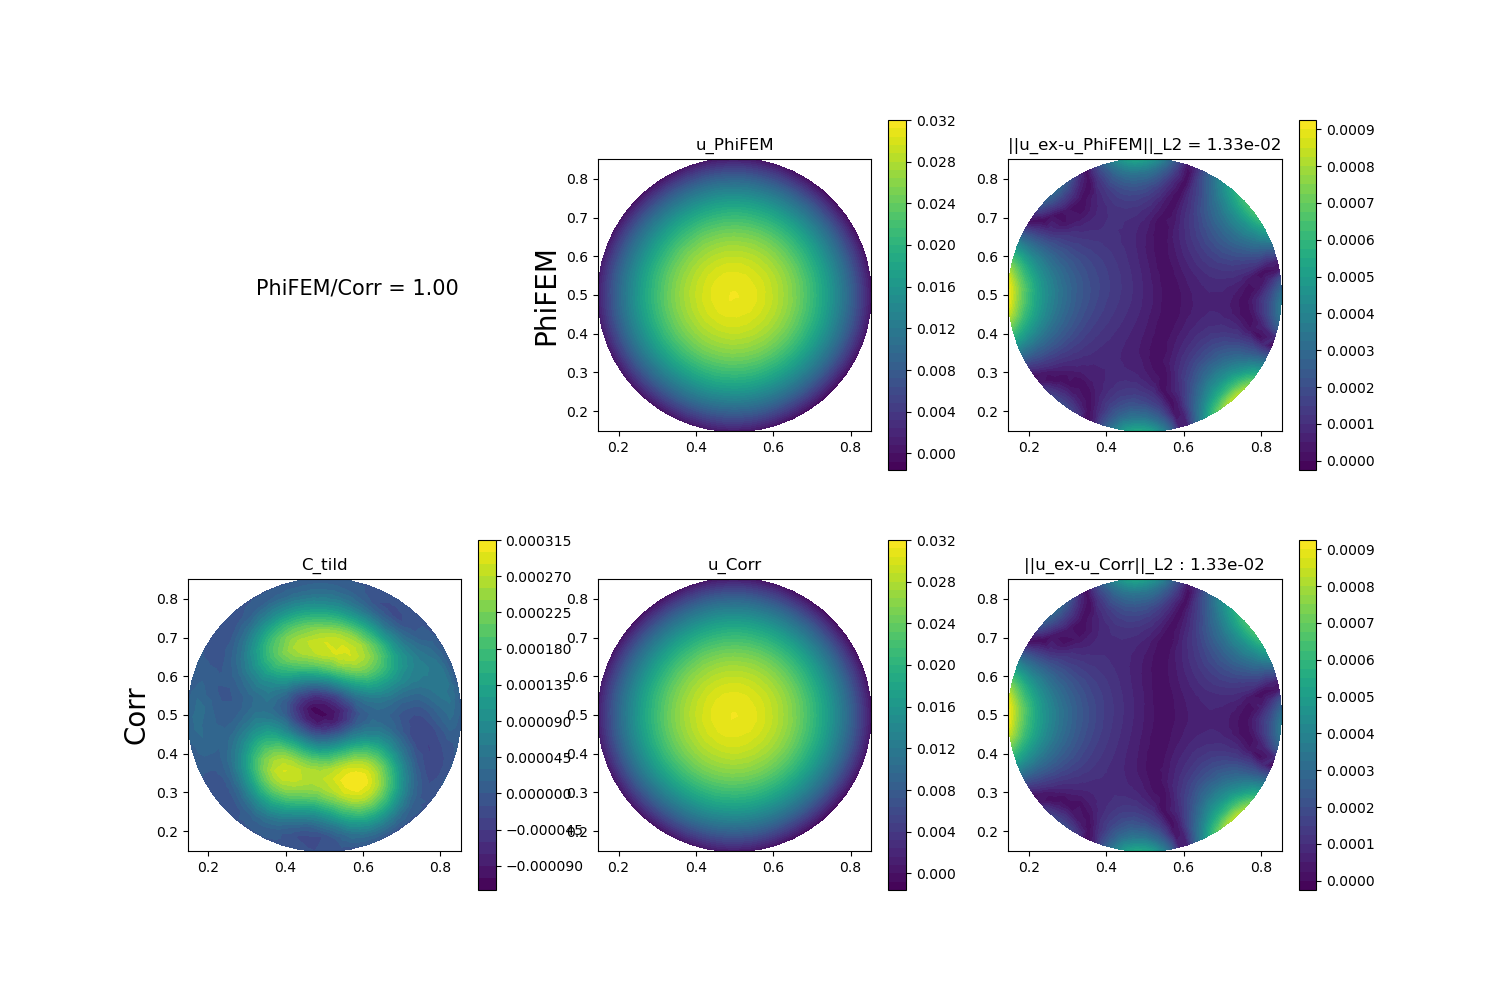
\includegraphics[width=0.6\linewidth]{"correction/bean/corr_PhiFEM_2_Omega.png"}
		\caption{Correction par addition avec $\phi$-FEM (projeté).}
	\end{figure}

	\newpage
	\textbf{Pumpkin :}
	
	\begin{figure}[H]
		\centering
		\includegraphics[width=0.6\linewidth]{"correction/pumpkin/corr_PhiFEM.png"}
		\caption{Correction par addition avec $\phi$-FEM.}
	\end{figure}
	
	\begin{figure}[H]
		\centering
		\includegraphics[width=0.6\linewidth]{"correction/pumpkin/corr_PhiFEM_Omega.png"}
		\caption{Correction par addition avec $\phi$-FEM (projeté).}
	\end{figure}

	\newpage
%	\section*{Bibliography}
	\printbibliography
\end{document}